%!TEX root = ../masters_thesis.tex


% requirements
%   geographical knowledge
%   contextualize / intersect historical sources
%   accept imprecision
%   prevent illusion of certainty

\section{User Interface Design Process} % (fold)
\label{sec:user_interface_design_process}

HistoGlobe is the application in which the work of this thesis is implemented. The Hivent Model presented in the section \ref{sec:hivent_model} serves as its data model and the methods to edit Hivent data in HistoGlobe (section \ref{sec:editing_hivent_data}) form parts of the computational model. However, developing the system bottom-up from the data model to the interface might not lead to usable system. Human Centered Design promotes a top-down process from the user via the interface into the core of the application. This section illustrates the iterative design process for this thesis seen in figure \ref{fig:human_centered_design}. The two main use cases for HistoGlobe that are focused in this thesis are:

\begin{compactenum}
  \item \textbf{Understanding} the history of countries.
  \item \textbf{Editing} the development of countries with historical changes by inserting forward and backwards operations and correcting wrong information in the system.
\end{compactenum}

The interviews with researchers in humanities at University of Virginia confirmed that the combination of a map and a timeline are a very appropriate and intuitive way to interactively visualize the history of countries. Thefore, the main concept of HistoGlobe introduced in section \ref{sec:histoglobe} does not need to be changed. This concept is extended by the \emph{HistoGraph} introduced in section \ref{sub:histograph}. This promising set of visualizations forms the \emph{Browsing Mode} of HistoGlobe to understand the history of countries.

For editing purposes the idea of a secod interface mode was developed: The \emph{Edit Mode} is the main product of the iterative design process illustrated in this section. It is based on the Edit Operations, the workflow to edit the data and the concepts of retrospective updates and backward operations from section \ref{sec:editing_hivent_data}. The Edit Mode allows to intuitively edit Hivents, Areas and operations directly in HistoGlobe, without the need to write data into tables or forms.

% - - - - - - - - - - - - - - - - - - - - - - - - - - - - - - - - - - - - - - -
\paragraph{Initial interviews} % (fold)
\label{par:initial_interviews}

Four researchers were asked about their opinions on the idea of HistoGlobe, use cases and the concept of the Edit Mode. The idea proved popular, especially for students and teachers in school, historically interested people in general and also for scholars in digital humanities. All researchers agreed that the key to a successful interface is usability, because editing data in time and space is a challenging task. A main concern is uncertainty: Almost all sorts of information in historical research -- temporal, spatial and thematic -- are potentially uncertain. A good user interface for researchers therefore has to support uploading historical sources and indicating uncertainty.

% paragraph initial_interviews (end)


% ------------------------------------------------------------------------------
\subsection{Paper Prototype} % (fold)
\label{sub:paper_prototype}

From the results of the inital interviews, an interface concept for the Edit Mode was developed in a paper prototype. It very fast to create and allows to identify flaws in the concept early in the design process. For this thesis, two paper prototype iterations were created that took about three full work days each: one day to create the prototype, half a day to conduct the study with three people, and one and a half days to analyze the results and rethink the concept.

\begin{figure}[H]
\centering
\begin{subfigure}{.5\textwidth}
  \centering
  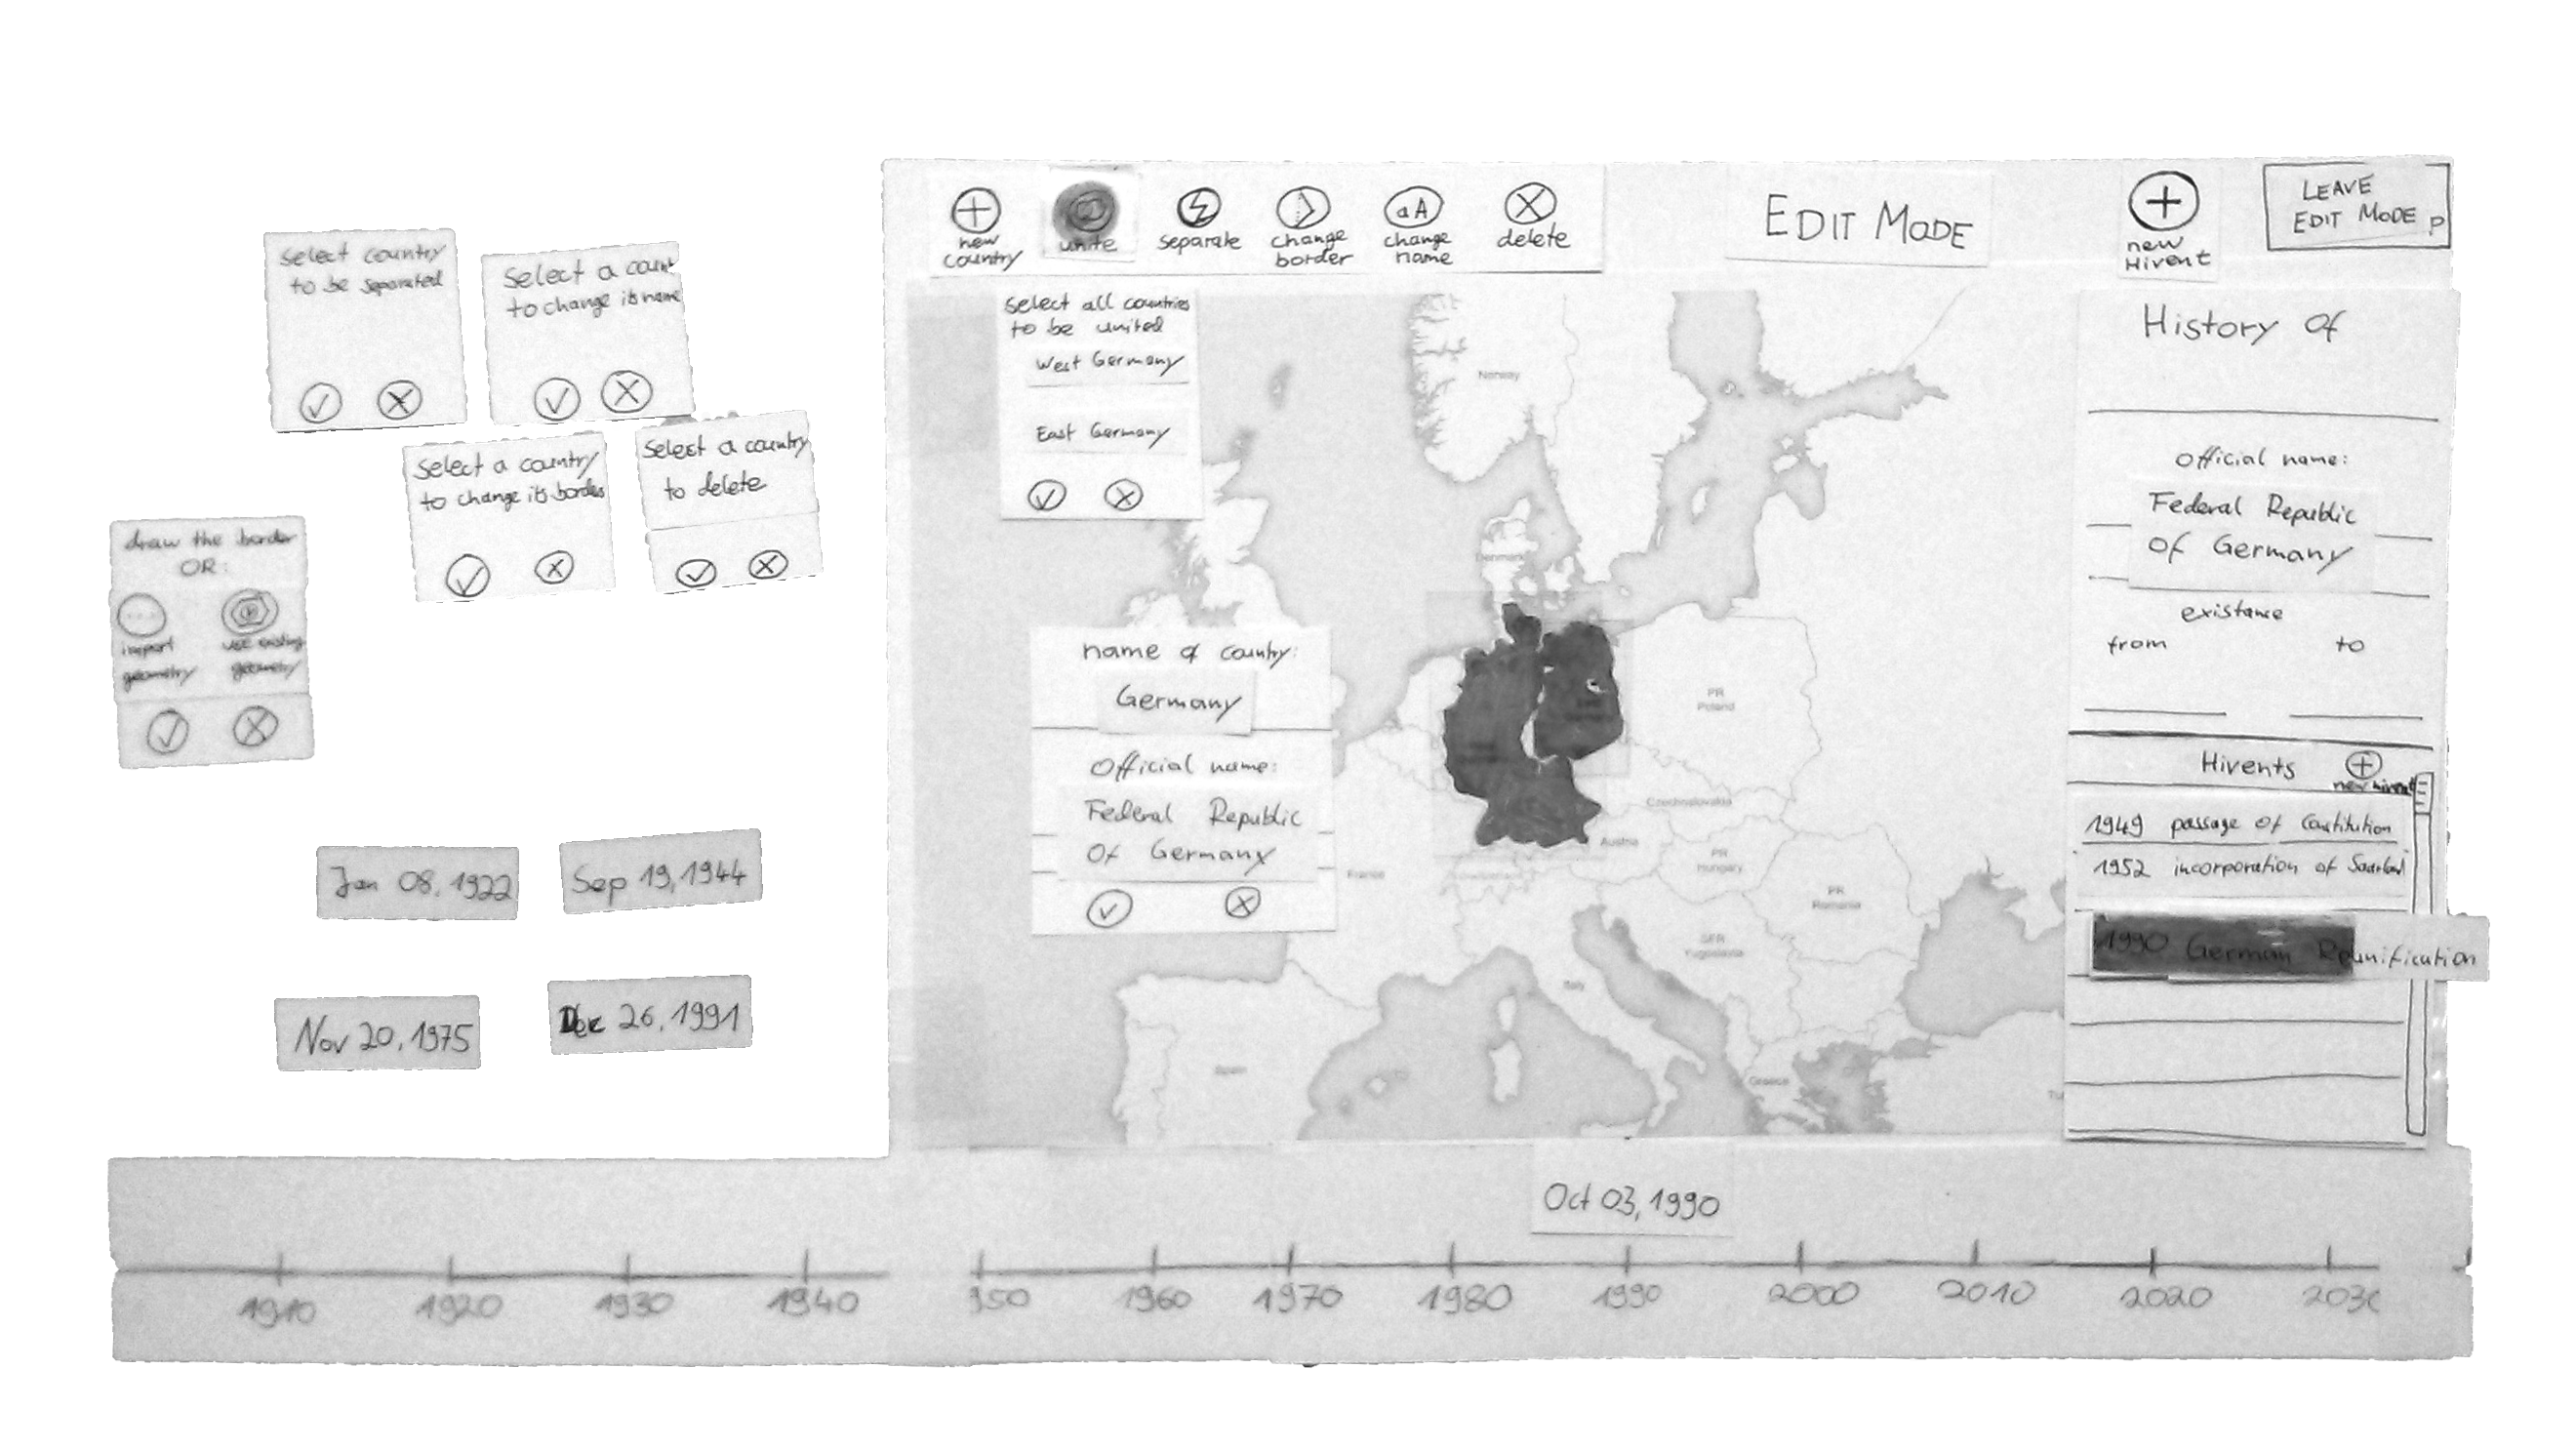
\includegraphics[width=225px]{graphics/development/user_interface_design_process/paper_prototype_1.png}
\end{subfigure}%
\begin{subfigure}{.5\textwidth}
  \centering
  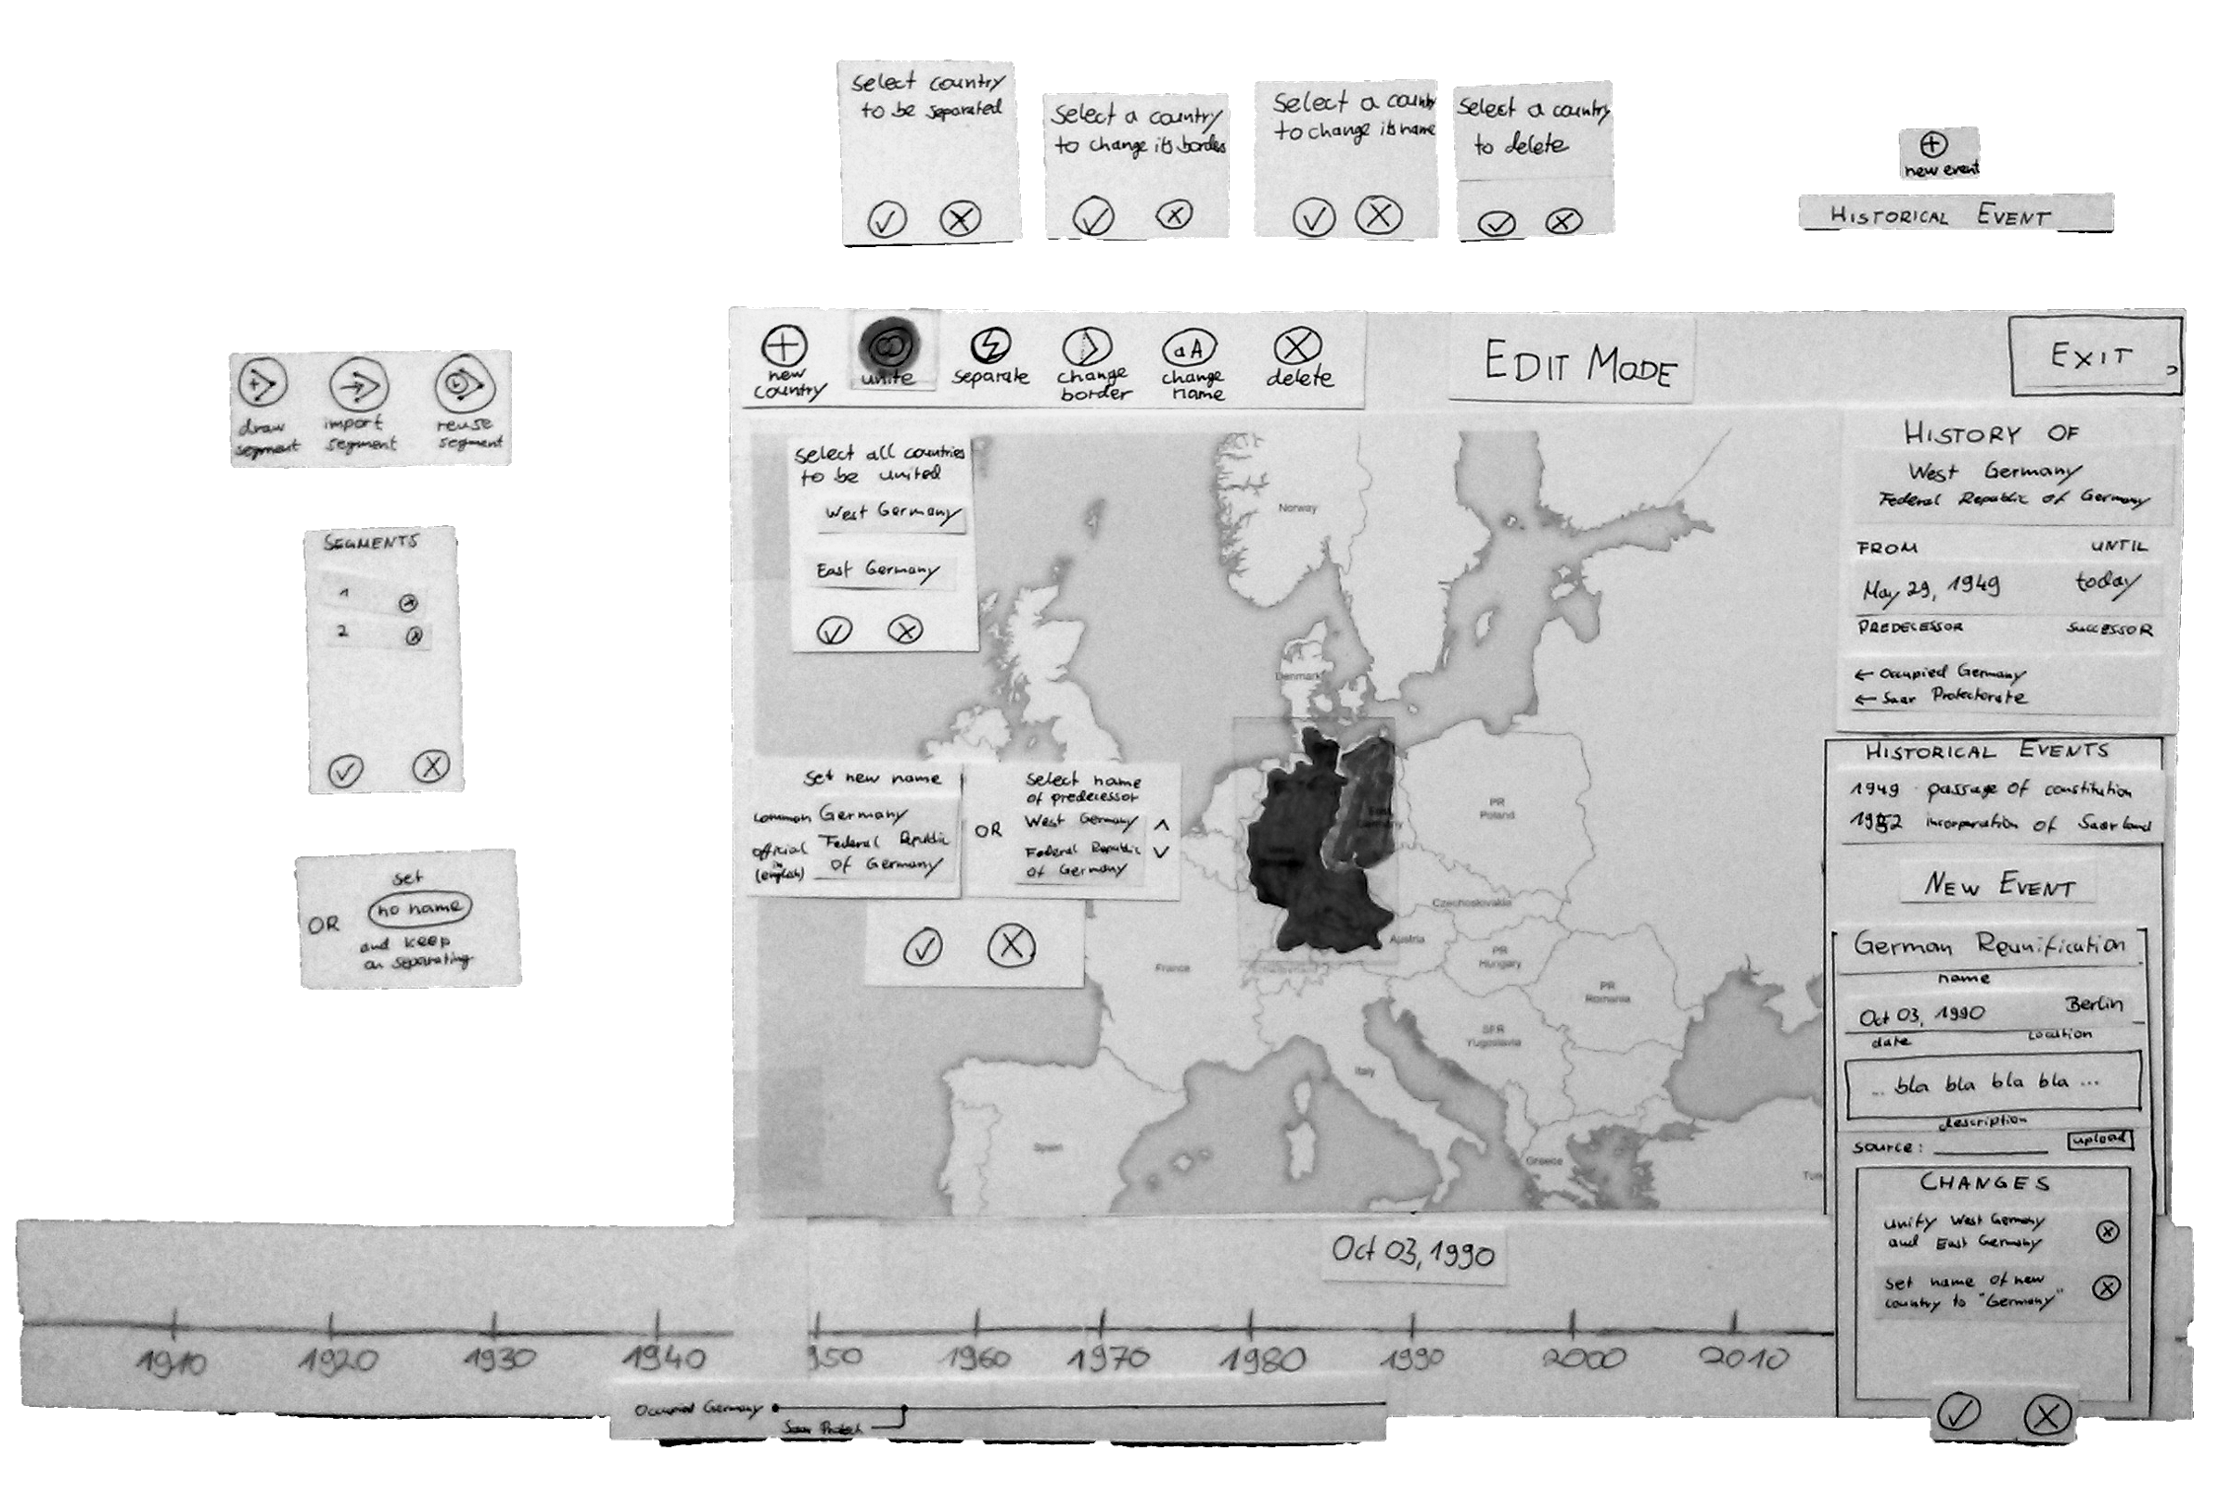
\includegraphics[width=225px]{graphics/development/user_interface_design_process/paper_prototype_2.png}
\end{subfigure}
\caption{The two iterations of the paper prototype for the Edit Mode}
\label{fig:paper_prototypes}
\end{figure}

The interface consists of a map of Europe, a timeline centered at 1975 and the buttons with a set of dialogs for the for the Edit Mode. Both prototypes were evaluated with three test subjects that had to solve four tasks covering different use cases and operations:
\begin{compactenum}
  \item 1300: Rename incorrectly spelled name of Switzerland on the map (\emph{correction})
  \item 1990: Unite East and West Germany (\emph{forward change})
  \item 1993: Separate the Soviet Union into Russia, Estonia, Latvia, etc. (\emph{forward change})
  \item 1944: Change the border between Finland and the Soviet Union before 1944 (\emph{backward change})
\end{compactenum}

Most parts of the interface concept were understood and all subjects could solve the first three tasks. However, there were also problems:

\begin{compactenum}
  \item There difference between Hivents, the history of a country and an historical change was unclear.
  \item The border drawing dialoge was imagined to be very complex.
  \item The backward change was not understood.
  \item Correcting the name Switzerland by changing the event that created it in 1300 caused confusion.
\end{compactenum}

The main finding of this step was that depending on the task, there is both an Hivent-based and an Area-based mental model of the task. This became apparent in the German Reunification Hivent: Some users started the unification operation first, and added West and East Germany afterwards -- and some selected first West Germany, then initiated a unification operation and then added East Germany. From that finding arose that the interface has to support both an Hivent-based and an Area-based approach to introduce historical changes and correct information on the map.

% subsection paper_prototype (end)

% - - - - - - - - - - - - - - - - - - - - - - - - - - - - - - - - - - - - - - -
\subsection{Mockup Prototype} % (fold)
\label{sub:mockup_prototype}

The main part of the design process was spent on the mockup prototypes. Their purpose is to rapidly develop an interface workflow that is understandable by the users. The prototypes were created in \emph{LibreOffice Impress}, an open-source slide-based presentation tool. The interface is simulated on slides: the map is a background image, the timeline, the set of buttons and dialogs for the Edit Mode and HistoGraph are modelled with geometric elements: lines, circles and rectangles. Interactivity is simulated by linking a click on an element to a different slide that shows the effect of the operation. This allows to model sudden changes in the interface.

\begin{figure}[ht]
  \centering
  \begin{subfigure}[b]{.5\textwidth}
    \centering
    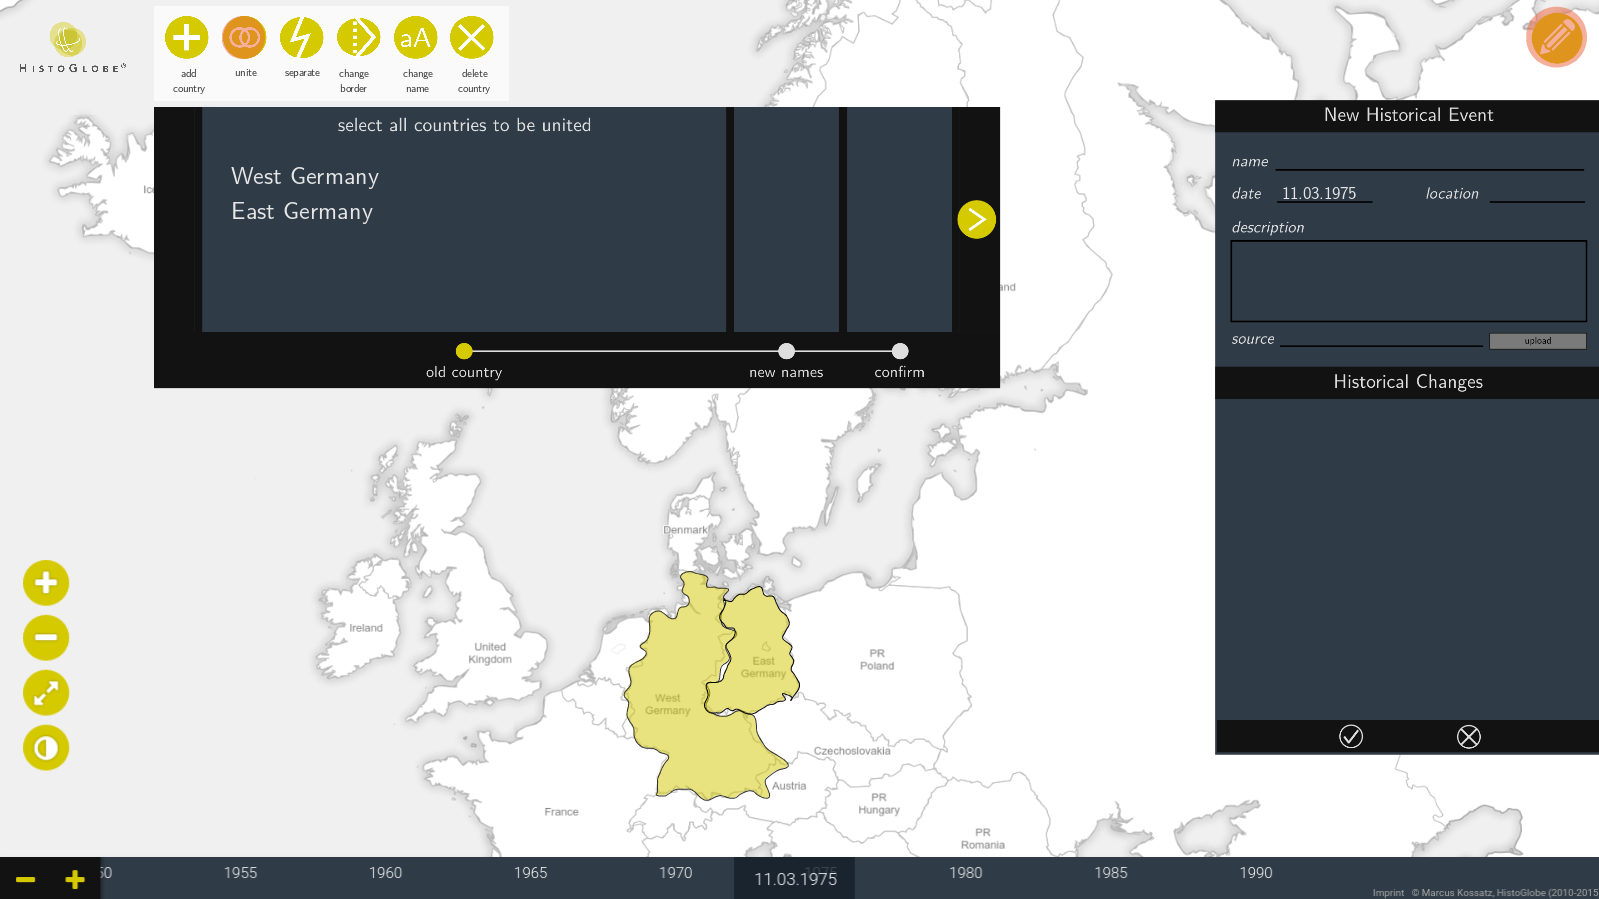
\includegraphics[width=180px]{graphics/development/user_interface_design_process/mockup_prototype_1.png}
  \end{subfigure}%
  \begin{subfigure}[b]{.5\textwidth}
    \centering
    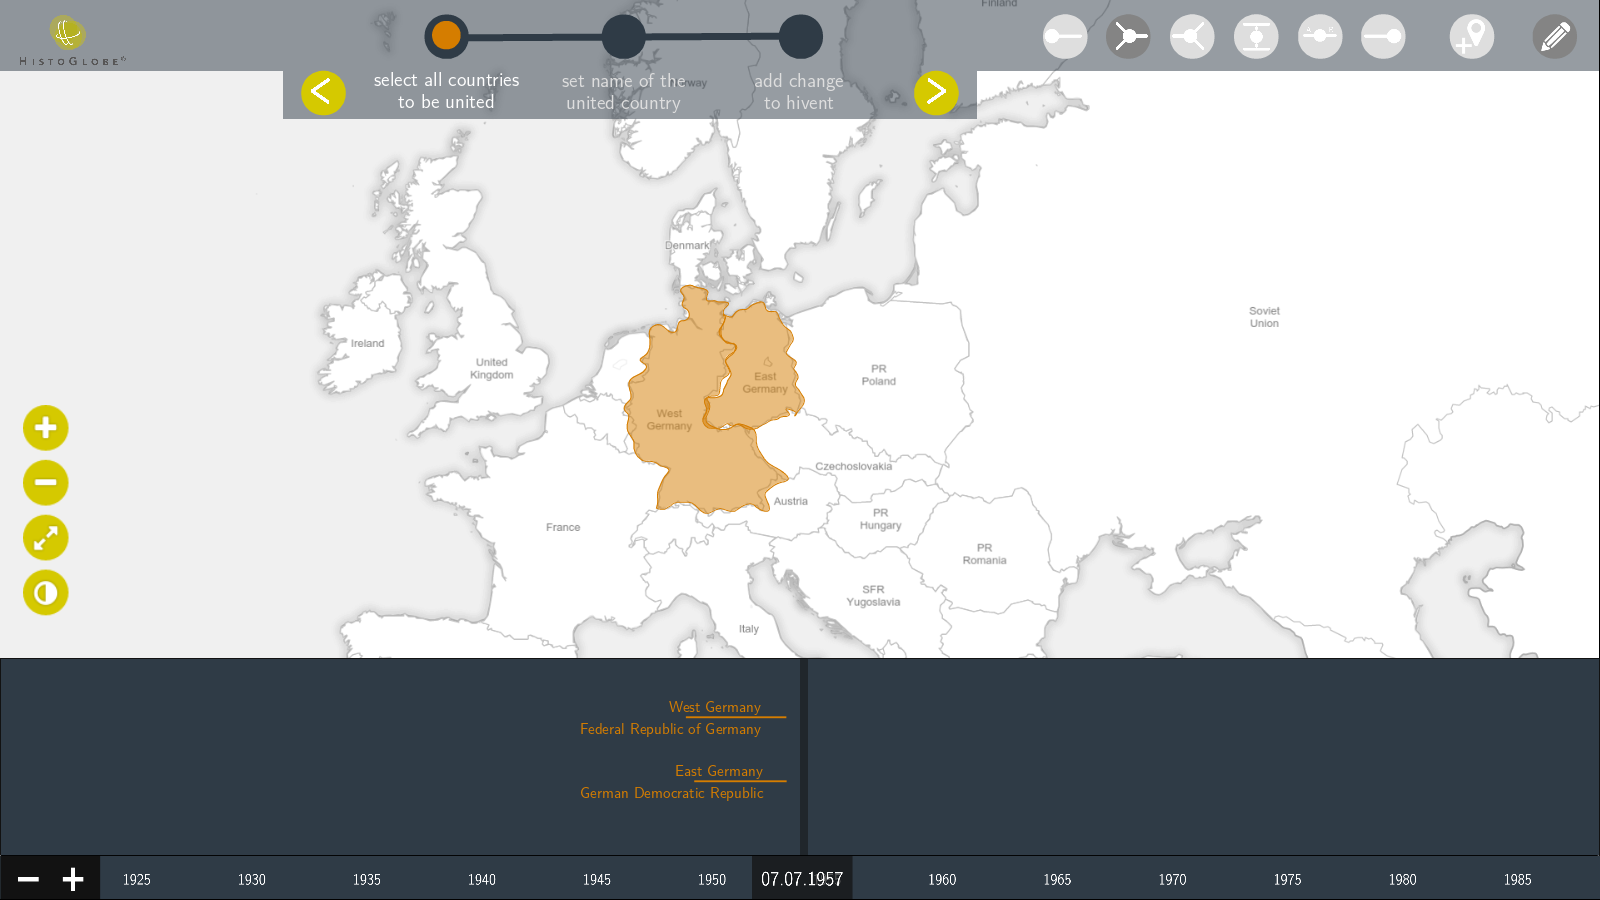
\includegraphics[width=180px]{graphics/development/user_interface_design_process/mockup_prototype_3.png}
  \end{subfigure} \\[0.8em]
  \caption{Two iteration stages of the mockup prototype for the Edit Mode}
  \label{fig:mockup_prototypes}
\end{figure}

Each prototype iteration was tested with multiple subjects and similar tasks as for the paper prototype. From one test to the next one changes to the interfaces were made. A lot of design problems, e.g. position of buttons, font sizes or color schemes were solved, but also conceptual issues arose.

\begin{quoteit}
  \begin{tabular}{l r}
    ``this was much easier than I thought'' ~~~~~~~~ &
    ``there is a training session needed'' \\[0.5em]
    ``the interface is very clear &
    ``the logic makes sense, \\
    and graphically pleasing'' &
    it is just very complex'' \\[0.5em]
    ``it's looking good'' &
    ``a nice tutorial and a good \\
    & documentation are necessary'' \\
  \end{tabular}
\end{quoteit}
\vspace{-1em}
\hfill -- interesting quotes from the users of the mockup prototype were:

Especially the problem to initiate a retrospective update and a backward backward change proved to be very difficult. There was a design solutions developed for each problem: For retrospective updates, the interface needs to provide a visual clue where the next potential conflict arises: Figure \ref{sfig:backward_change} shows that West Germany can only be active until 1990, because then present-day Germany uses its territory. For backward operations a button that flippes an Edit Operation  is introduced in figure \ref{sfig:backward_change}: the \texttt{SEC} operation introduced to secede East Germany from Germany will be flipped into an \texttt{INC} operation to incorporate East Germany into Germany. The two grey Hivent markers on the left side of the timeline indicate that West and East Germany need a creation event, otherwise they would be active backwards all the way to $t_0$, the initial state of the system.

\begin{figure}[ht]
\centering
\begin{subfigure}[b]{.5\textwidth}
  \centering
  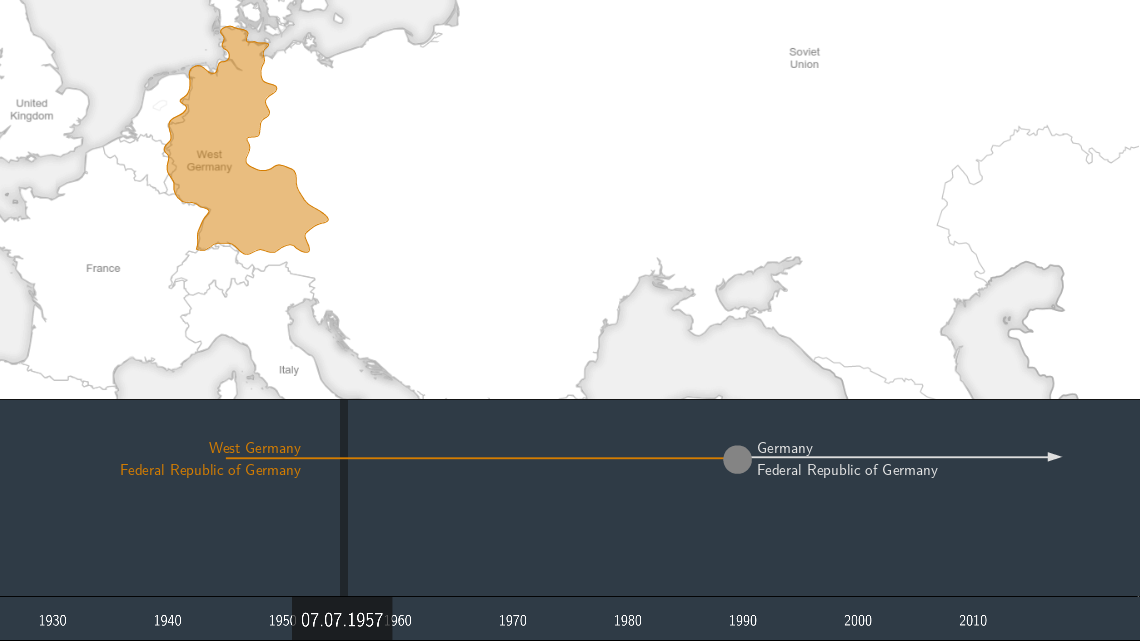
\includegraphics[width=200px]{graphics/development/user_interface_design_process/retrospective_update.png}
  \caption{Retrospective updates: Visualizing the next conflict}
  \label{sfig:retrospective_update}
\end{subfigure}%
\begin{subfigure}[b]{.5\textwidth}
  \centering
  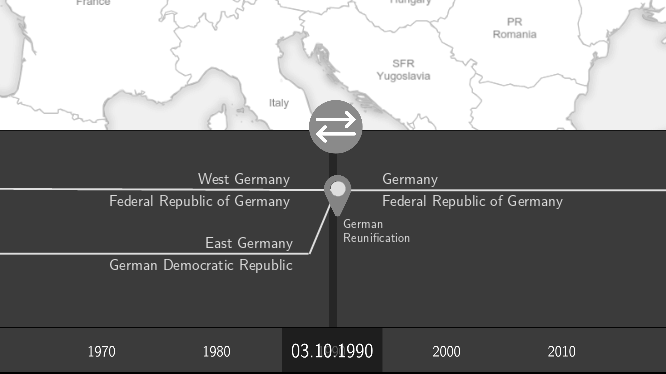
\includegraphics[width=200px]{graphics/development/user_interface_design_process/backward_change.png}
  \caption{Backward operation: flipping the Edit Operation}
  \label{sfig:backward_change}
\end{subfigure}
% \caption{Two approaches for editing changes backwards}
\label{fig:backward_change}
\end{figure}

The prototype was very valuable for the development process. In a total of two weeks, an interface concept and workflow was designed thatwas understandable by the users. Its creation took longer than the paper prototype, but was much faster than implementing an interactive Web-based interface.


% subsection mockup_prototype (end)

% - - - - - - - - - - - - - - - - - - - - - - - - - - - - - - - - - - - - - - -
\subsection{Web-based prototype} % (fold)
\label{sub:web_based_prototype}

The main advantage of the design process so far is that it prevents major redesigns of the final Web-based prototype. After three months of implementation of the final system, the interface looks very similar to the last version of the mockup prototype. The main elements of the interface are the map, the timeline with the Now Marker the control buttons the map and the timeline and the Edit Mode. However, not all desired features could be implemented: For the HistoGraph there were too many conceptual problems mentioned in section \ref{sub:histograph} that have to be solved first. Backward operations and retrospective updates are not supoprted as well, because of their complex nature. The HistoGlobe version developed in this thesis supports editing the development of countries with forward operations at the end of the timeline. The interaction and behavior is introduced in this section at the example of the fictional secession of Scotland from the United Kingdom in 2018.

\newpage
\begin{minipage}[t]{0.47\textwidth}

  \begin{figure}[H]
    \centering
    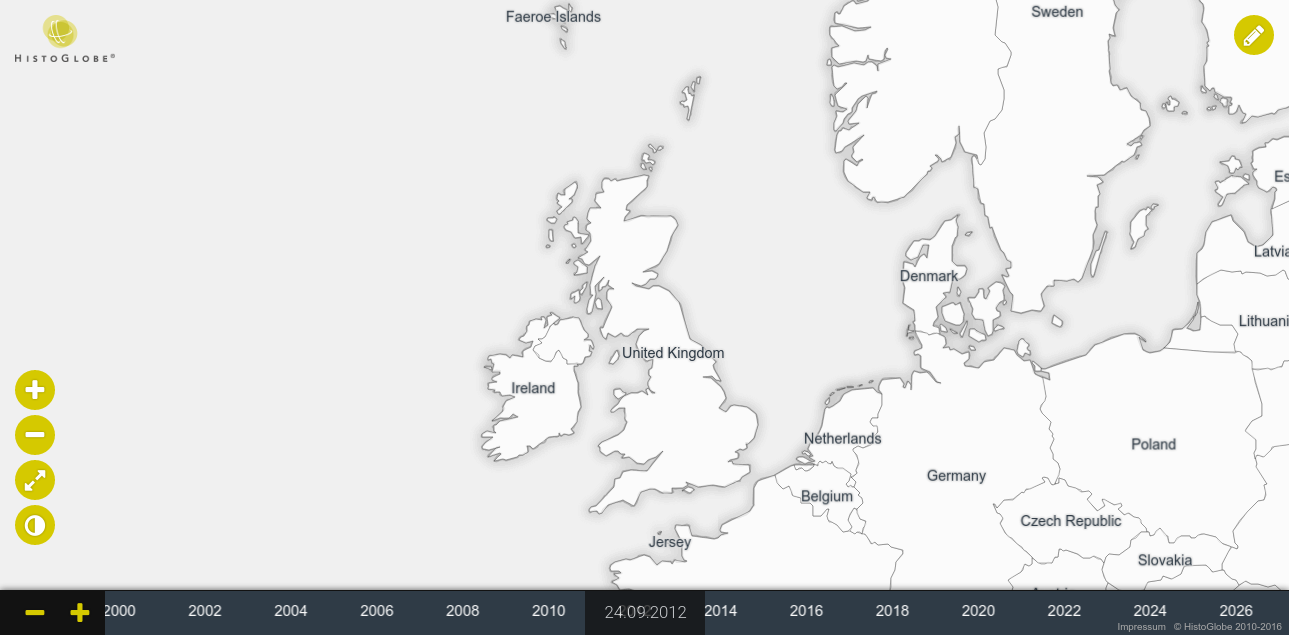
\includegraphics[width=1.0\textwidth]{graphics/development/user_interface_design_process/1_init.png}
    \caption{Initial state of the Browsing Mode}
    \label{fig:final_1_init}
  \end{figure}

  The initial state of the user interface. Additional to the original elements, there is an edit button on the upper right corner. Clicking it enters the Edit Mode of the system.

\end{minipage}    % N.B. the % is very important
\hspace{1.5em}    % N.B. this must go in this line, no blank lines !!!
\begin{minipage}[t]{0.47\textwidth}

  \begin{figure}[H]
    \centering
    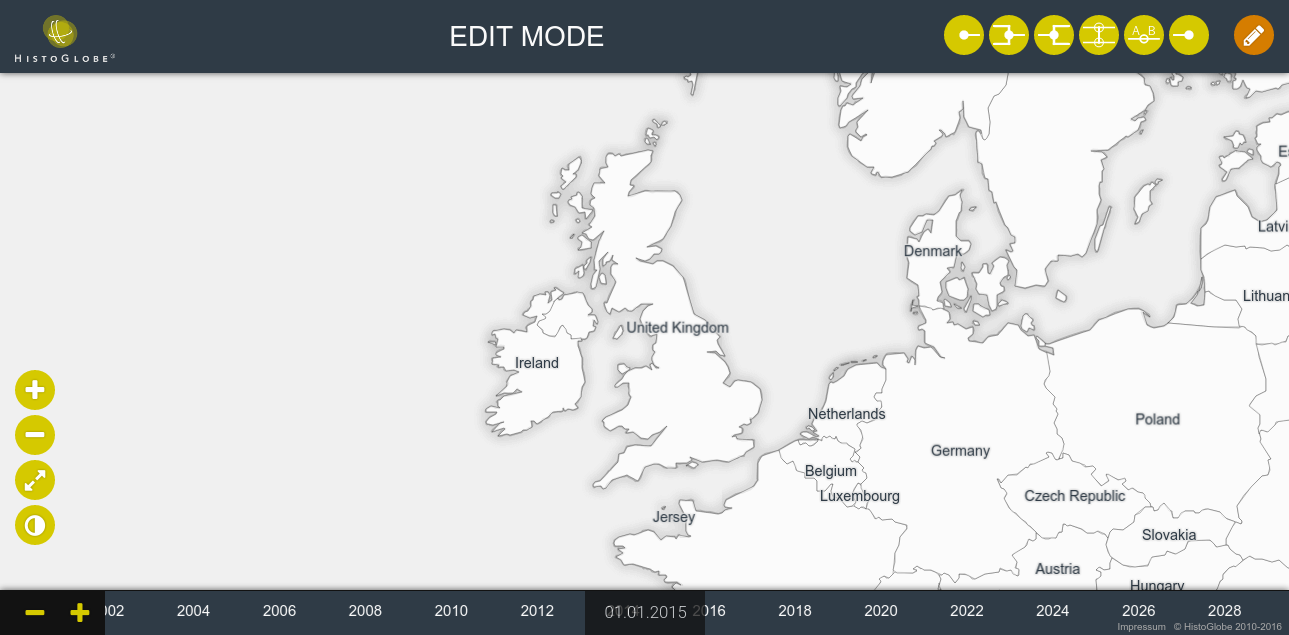
\includegraphics[width=1.0\textwidth]{graphics/development/user_interface_design_process/2_edit_mode.png}
    \caption{Initial state of the Edit Mode}
    \label{fig:final_2_edit_mode}
  \end{figure}

  In the Edit Mode, a title bar and six buttons for the Edit Operations are   revealed. Clicking a button starts the operation workflow introduced in section \ref{sub:edit_workflow}.

\end{minipage}

\vspace{1em}
\begin{minipage}[t]{0.47\textwidth}

  \begin{figure}[H]
    \centering
    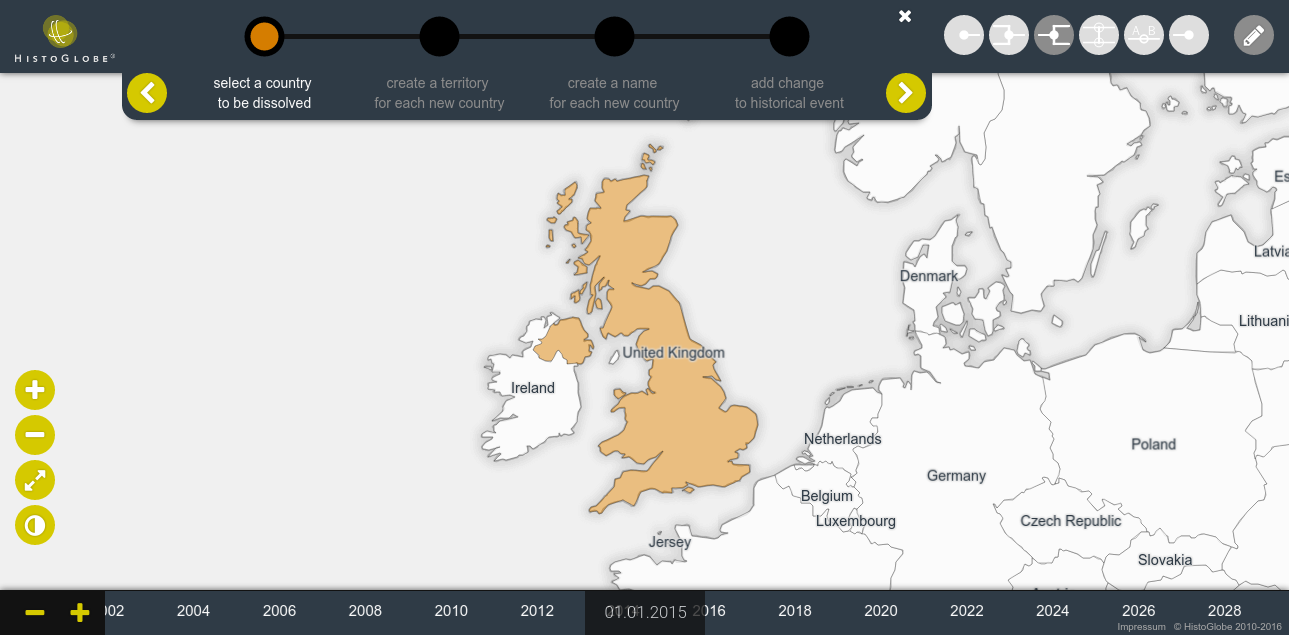
\includegraphics[width=1.0\textwidth]{graphics/development/user_interface_design_process/3_select_old_areas.png}
    \caption{1) Select old Areas}
    \label{fig:final_3_select_old_areas}
  \end{figure}

  A \emph{Workflow Window} guides the user step-by-step through the process of completing the Edit Operation. In the case of \texttt{DIS}, the user has to select the country to be dissolved by clicking it on the map. After the step is completed, clicking the next button in the workflow window procceeds to the next step. At each point in the workflow, clicking the back button reverts the previous action.

\end{minipage}    % N.B. the % is very important
\hspace{1.5em}    % N.B. this must go in this line, no blank lines !!!
\begin{minipage}[t]{0.47\textwidth}

  \begin{figure}[H]
    \centering
    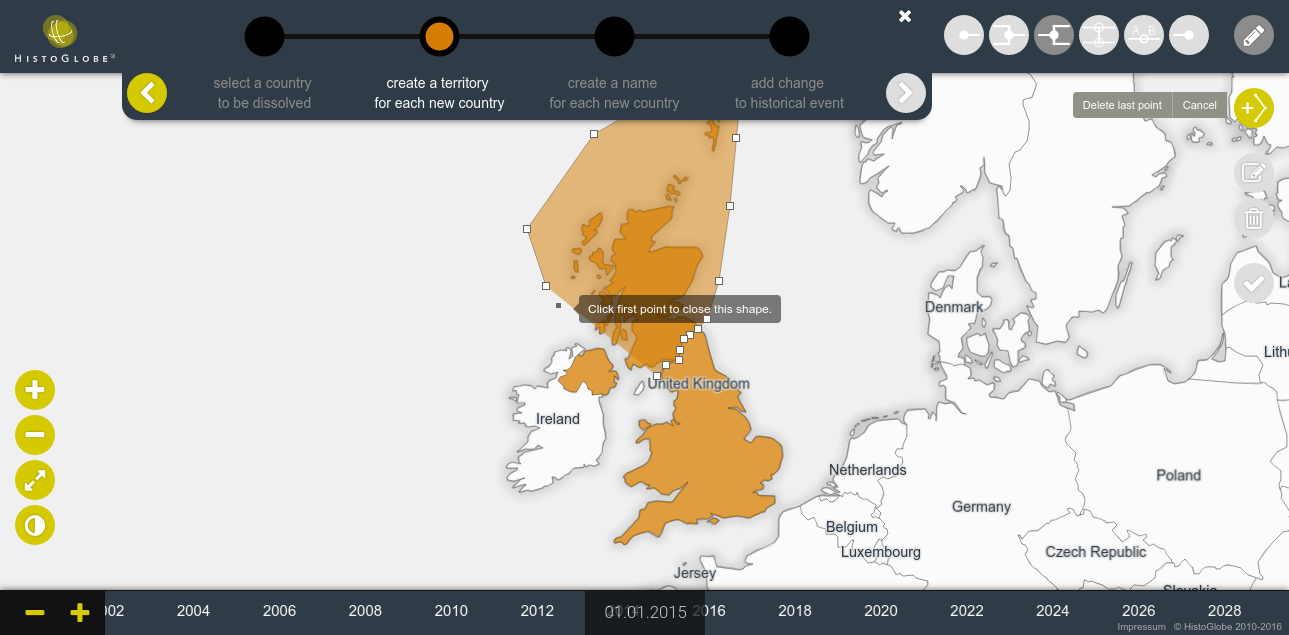
\includegraphics[width=1.0\textwidth]{graphics/development/user_interface_design_process/4_set_new_territories.png}
    \caption{2) Set a new territory}
    \label{fig:final_4_set_new_territories}
  \end{figure}

  In step two, the user has to create a territory for each new Area. The \emph{New Territory Tool} provides the functionality to create, manipulate and delete polygons directly on the map. The drawn polypolygon is intersected with the old territory to create the new Area. After at least one new territory is created sucessfully, the remaining old territory can be selected on the map to be used as the last territory. If the whole old territory is distributed among the new Areas, the workflow proceeds to the next step.

\end{minipage}

\vspace{1em}
\begin{minipage}[t]{0.47\textwidth}

  \begin{figure}[H]
    \centering
    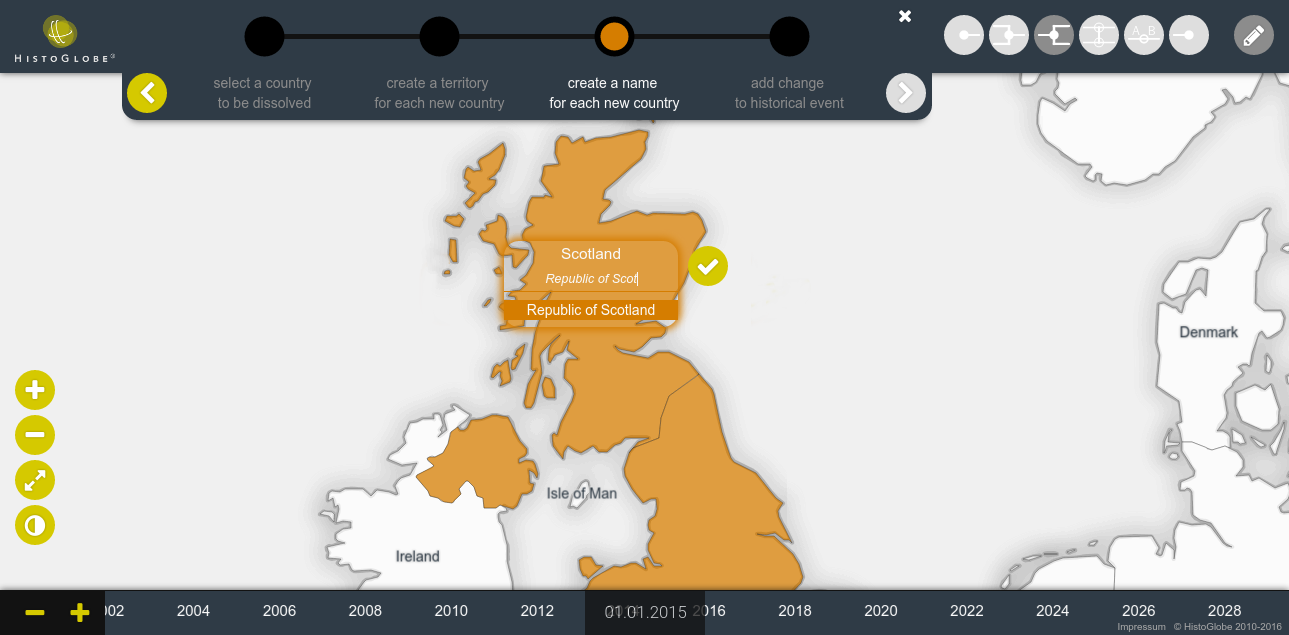
\includegraphics[width=1.0\textwidth]{graphics/development/user_interface_design_process/5_set_new_name.png}
    \caption{3) Set a new name}
    \label{fig:final_5_set_new_name}
  \end{figure}

  In the next step, the user has to define a name for each Area that has just been created. The \emph{New Name Tool} is a draggable box with two lines for the short and formal name. Via instant search, the user can select existing country names from the database to be put in. When clicking the confirm button, the short name is put directly on the map.

\end{minipage}    % N.B. the % is very important
\hspace{1.5em}    % N.B. this must go in this line, no blank lines !!!
\begin{minipage}[t]{0.47\textwidth}

  \begin{figure}[H]
    \centering
    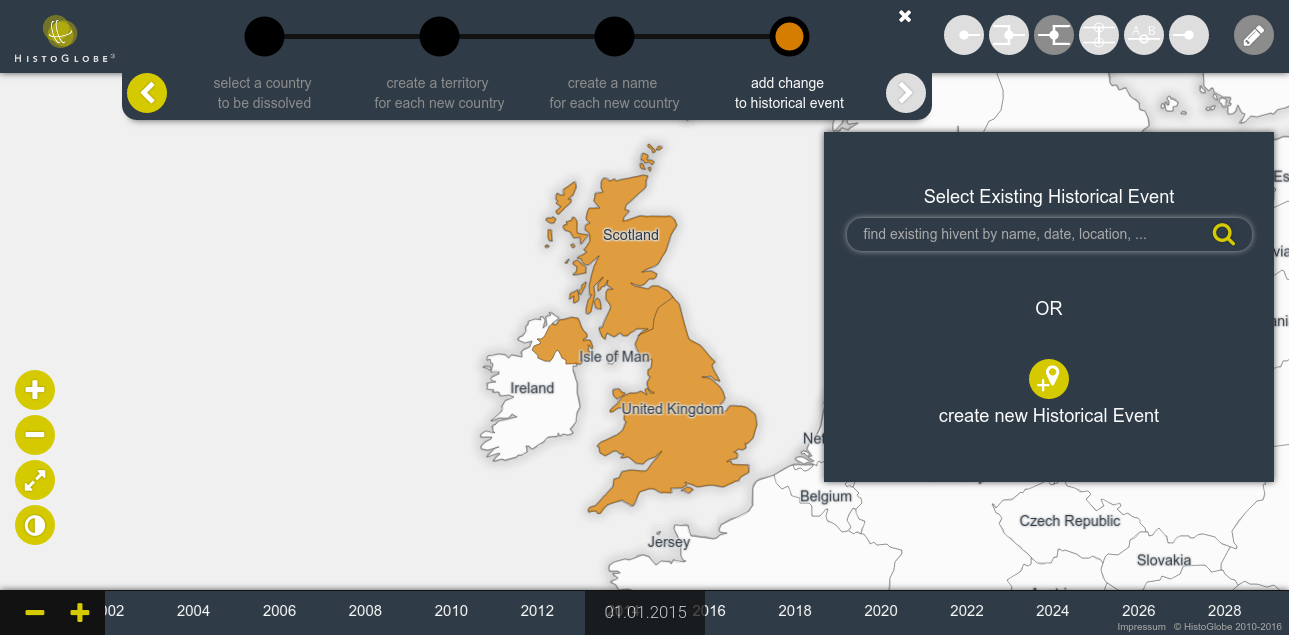
\includegraphics[width=1.0\textwidth]{graphics/development/user_interface_design_process/6_add_change_to_hivent_1.png}
    \caption{4) Add the Operation to a Hivent}
    \label{fig:final_6_add_change_to_hivent_1}
  \end{figure}

  When all names are set, the Edit Operation is complete. In the last step of the workflow, it has to be added to an Hivent. The \emph{New Hivent Box} offers two possibilities: search for an existing Hivent and add the operation to it or create a new Hivent.

\end{minipage}

\vspace{1em}
\begin{minipage}[t]{0.47\textwidth}

  \begin{figure}[H]
    \centering
    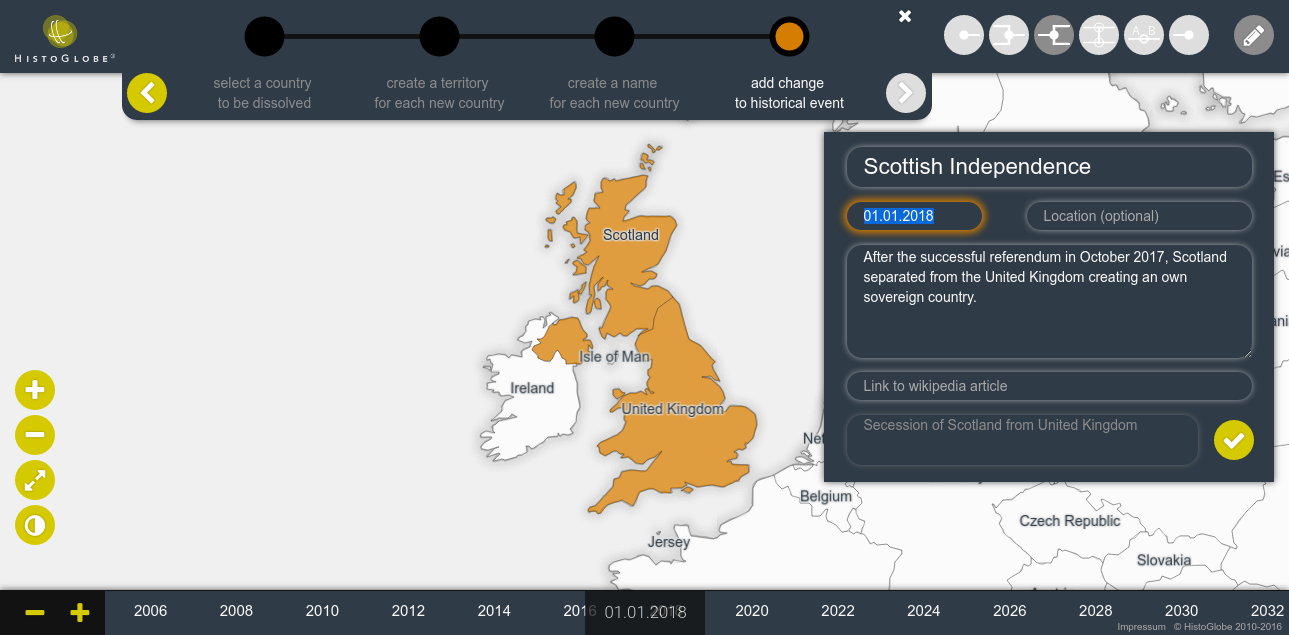
\includegraphics[width=1.0\textwidth]{graphics/development/user_interface_design_process/7_add_change_to_hivent_2.png}
    \caption{4) Create a new Hivent}
    \label{fig:final_7_add_change_to_hivent_2}
  \end{figure}

  The new Hivent created for that change is the ``Scottish Independence'' on 01.01.2018 with a description of the Hivent and possibly a location and a link to a wikipedia article. In the last line, the historical change ``Secession of Scotland from the United Kingdom'' is noted. Clicking the confirm button finalizes the workflow.

\end{minipage}    % N.B. the % is very important
\hspace{1.5em}    % N.B. this must go in this line, no blank lines !!!
\begin{minipage}[t]{0.47\textwidth}

  \begin{figure}[H]
    \centering
    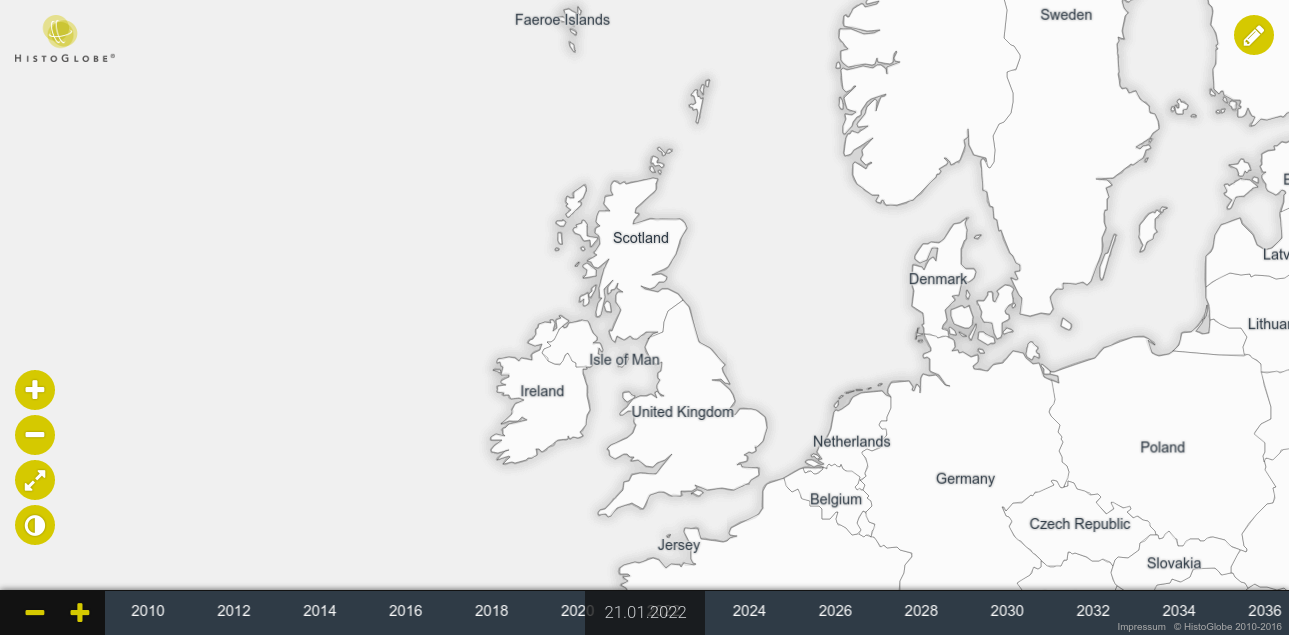
\includegraphics[width=1.0\textwidth]{graphics/development/user_interface_design_process/8_final_state.png}
    \caption{The final state with Scotland}
    \label{fig:final_8_final_state}
  \end{figure}

  Clicking the edit button again leaves the Edit mode back to the Browsing Mode. Scotland and the United Kingdom are visible as separate Areas on the map after 2018. When moving the timeline before 2018, Scotland is still part of the UK.

\end{minipage}

% subsection web_based_prototype (end)

% section user_interface_design_process (end)